\section{Experiment Setup}
\subsection{Motivation}

During Automated Program Repair (APR) activities, traditional methods (based on heuristics or templates) often generate syntactically correct changes, but they fall short in the semantic and code style aspects (insert ref).

In this context, Large Language Models (LLMs) are capable of capturing code patterns and semantic context with high precision.
On the other hand, LLMs exhibit significant sensitivity to how their instructions (prompts) are phrased. Different instructions can alter the fidelity to the original style, the clarity of the patch, and the size of the modification, especially if little context is provided during the correction process (insert ref).

\subsection{Dataset}

The experiment uses the Pytracebugs dataset \cite{Pytracebugs}, which contains Python source codes from GitHub repositories at the granularity of function snippets and their corresponding Traceback errors; see the example below.


\begin{figure}[h!]
    \centering
    \caption{An example of a single data point from the Pytracebugs dataset.}
    \label{fig:dataset-example}

    % (a) The Buggy Code
    \begin{lstlisting}[
        language=Python,
        frame=single,
        basicstyle=\ttfamily\small,
        caption={a) Buggy Code Snippet (\texttt{before\_merge})},
        belowcaptionskip=-0.5em % Adjust spacing
        ]
def noise(self, value):
  self.noise_covar.initialize(value)
    \end{lstlisting}

    % (b) The Traceback Error
    \begin{lstlisting}[
        frame=single,
        basicstyle=\ttfamily\small,
        caption={b) Traceback Error (\texttt{full\_traceback})},
        belowcaptionskip=-0.5em % Adjust spacing
        ]
import gpytorch
gl = gpytorch.likelihoods.GaussianLikelihood()
gl.initialize(noise=1)
Traceback (most recent call last):
File ""<stdin>"", line 1, in <module>
File "".../gpytorch/gpytorch/module.py"", line 89, in initialize
setattr(self, name, val)
File ""../lib/python3.6/site-packages/torch/nn/modules/module.py"", line 579, in __setattr__
object.__setattr__(self, name, value)
File "".../gpytorch/gpytorch/likelihoods/gaussian_likelihood.py"", line 63, in noise
self.noise_covar.initialize(value)
TypeError: initialize() takes 1 positional argument but 2 were given
    \end{lstlisting}

    % (c) The Fixed Code
    \begin{lstlisting}[
        language=Python,
        frame=single,
        basicstyle=\ttfamily\small,
        caption={c) Fixed Code Snippet (\texttt{after\_merge})}
        ]
def noise(self, value):
  self.noise_covar.initialize(noise=value)
    \end{lstlisting}
\end{figure}

\begin{figure}[h!]
    \centering
    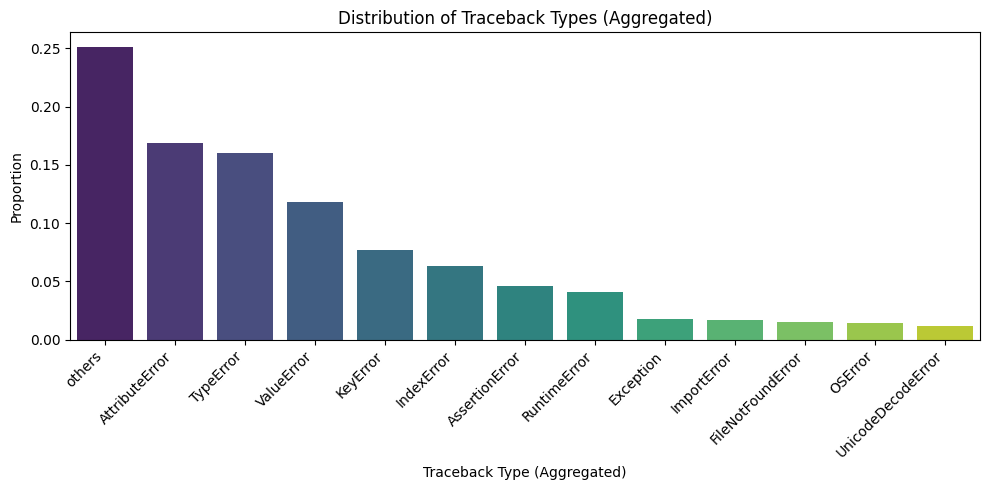
\includegraphics[width=0.7\textwidth]{Cap2/dataset-traceback-type.png}
    \caption{Distribution of Error Types in the dataset - Less than 1\% relevant are consolidated into 'others' category.}
    \label{fig:dataset-traceback-types}
\end{figure}

Most frequent traceback errors can be found in Figure \ref{fig:dataset-traceback-types}, with the most frequent ones being Atribute Error and TypeError with $16.84\%$ and $16\%$ of the values respectivelly. Also, there is a significant amount of erros that appear less than $1\%$ of the time, and were aggregated into the 'Others' Category.

%TODO: Adicionar exemplos de trabalhos publicados que utilizam como referencia o dataset proposto.
Some published works that use this dataset aim to study problems such as Vulnerability Detection \cite{zhao2024coding} and fault localization \cite{kulkarni2024graph}.

\subsection{LLM Models}
For the first experiment, four models were chosen. Two of these are open-source models specialized in code generation, considered state-of-the-art in this category: Qwen 2.5 coder 32b (instruct) \cite{hui2024qwen25codertechnicalreport} and Codestral 2501 \cite{Codestral_202501}. Additionally, two state-of-the-art, commonly used closed-source models of a relatively similar size were selected: Claude $3.5$ Sonnet and GPT $4o$ Model.

Although these models are all similarly competitive in structured benchmarks, they differ considerably in terms of usage cost. For reference, the token cost for each selected model is shown in Table \ref{tab:model-tokens}.
\begin{table}[h!]
\centering
\caption{Token usage price per model.}
\label{tab:model-tokens}
\begin{tabular}{|l|c|c|}
\hline
\textbf{Model} & \textbf{Input Tokens (1M)} & \textbf{Output Tokens (1M)} \\ \hline
Claude Sonnet 3.5 & \$3.0 & \$15.0 \\ \hline
Gpt 4o & \$2.5 & \$10 \\ \hline
Codestral 2501 & \$0.3 & \$0.9 \\ \hline
Qwen 2.5 Coder 32B Instruct & \$0.05 & \$0.20 \\ \hline
\end{tabular}
\end{table}
% todo addicionar gemini flas
%TODO melhorar a argumentação desses modelos
% Falar do tamanho dos modelos e da comparabilidade deles. Exibir ranking. Existem muitos, portanto qualquer escolha tem uma arbitrariedade. Não vamos todos no hugging faces.

% TODO trazer artigos que divulgam esses modelos.


\subsection{Prompts updated}

To test the model's sensitivity to the prompt's instructions, all prompts were formatted 
using a consistent template, shown in Listing \ref{lst:prompt-template}. This structure ensures 
that each model receives the context—buggy code and traceback error—in a clear, delimited 
format, and is explicitly asked to return only the corrected code.

% The 'figure' environment helps manage the placement and captioning of the listing.
\begin{figure}[h!]
% This is the crucial line that starts the code block.
% The formatting options are placed in the square brackets.
\begin{lstlisting}[
    caption={The general template used for all prompts.},
    label={lst:prompt-template},
    basicstyle=\ttfamily\small,
    frame=single,
    breaklines=true
]
{{ instruction_prompt }}

### BUGGY CODE:
{{ buggy_code }}

### ERROR:
{{ traceback_error }}

### RETURN ONLY THE CORRECTED CODE BELOW:

IMPORTANT: Return ONLY the corrected/requested code. Do not include any explanations, comments about the changes, or other text. Just return the pure code.

\end{lstlisting} % This line correctly ends the code block.
\end{figure}
% It clearly isolates the variable you are testing.
\begin{table}[h!]
\centering
\caption{Instruction variations for the \texttt{instruction\_prompt} variable.}
\label{tab:prompt-instructions}
\begin{tabular}{|l|p{0.55\textwidth}|p{0.15\textwidth}|}
\hline
\textbf{Prompt ID} & \textbf{Instruction Text} & \textbf{System Prompt} \\ \hline
P1 (Baseline) & You are a helpful assistant that corrects the code based on the traceback error. & False. \\\hline
P2 (Style-aware) & You are a helpful assistant that corrects the code based on the traceback error. You must respect the original code structure and the original code style. & False. \\ \hline
P3 (System Prompt) & You are a helpful assistant that corrects the code based on the traceback error. & True. \\ \hline
\end{tabular}
\end{table}
The core of the experiment lies in the variation of the \texttt{instruction\_prompt} placeholder and the addition of system prompt. 
We designed three distinct instructions, which we will refer to as P1 (Baseline) and P2 (Style-aware) and P3 (System Prompt), 
to evaluate the impact of a more detailed directive. The specific text for each instruction 
is detailed in Table \ref{tab:prompt-instructions}.

\subsection{Experiment tracking}
For each of the 4 models, 300 responses were executed for each of the prompts, totaling 4 x 300 x 3 = 3600 responses. For each response, the following metrics were evaluated: AST, AST-Normalized, CodeBLEU, N-gram match, Weighted N-gram match, Dataflow Match.
Each metric was compared against both the original (buggy) code and the ground truth correction.


\subsection{Implementation Details}
\label{sec:implementation-details}

All API calls to the proprietary models (GPT-4o and Claude 3.5 Sonnet) and the open-source models (Qwen 2.5 and Codestral) were managed through the \textbf{OpenRouter} API aggregation service. This approach was chosen to ensure a consistent and reproducible experimental setup across all models from a single interface.

The specific model identifiers used on the platform are listed below. To ensure that the results were as deterministic as possible and to facilitate a fair comparison, the generation parameters were kept constant for all API calls: a \textbf{temperature of 0} and a \textbf{top\_p of 1.0} were used. All experiments were conducted in \textbf{July 2025}.

\begin{itemize}
    \item \texttt{openai/gpt-4o}
    \item \texttt{anthropic/claude-3.5-sonnet}
    \item \texttt{qwen/qwen-2.5-coder-32b-instruct} 
    \item \texttt{mistralai/codestral-2501}
\end{itemize}

\subsubsection{Experimental Results Summary}
Table \ref{tab:comprehensive-results} presents the comprehensive results of our experiment, showing the performance of all four models across the three prompt conditions for each evaluation metric. The results are formatted as mean ± standard deviation to provide both central tendency and variability measures.

\begin{table}[h!]
\centering
\caption{Comprehensive metrics comparison across all models and prompt conditions (mean ± std).}
\label{tab:comprehensive-results}
\resizebox{\textwidth}{!}{%
\begin{tabular}{|l|l|c|c|c|c|c|c|c|c|}
\hline
\textbf{Model} & \textbf{Prompt} & \textbf{AST Score} & \textbf{Text Score} & \textbf{AST Norm.} & \textbf{CodeBLEU} & \textbf{N-gram} & \textbf{W. N-gram} & \textbf{Syntax} & \textbf{Dataflow} \\
\hline
\multirow{3}{*}{Claude 3.5 Sonnet} & Baseline & $0.22 \pm 0.36$ & $0.68 \pm 0.23$ & $0.29 \pm 0.40$ & $0.73 \pm 0.17$ & $0.64 \pm 0.27$ & $0.71 \pm 0.24$ & $0.76 \pm 0.19$ & $0.71 \pm 0.26$ \\
\cline{2-10}
& Style-aware & $0.23 \pm 0.37$ & $0.69 \pm 0.23$ & $0.31 \pm 0.41$ & $0.73 \pm 0.17$ & $0.64 \pm 0.26$ & $0.72 \pm 0.24$ & $0.77 \pm 0.19$ & $0.71 \pm 0.26$ \\
\cline{2-10}
& System & $0.23 \pm 0.36$ & $0.71 \pm 0.22$ & $0.38 \pm 0.44$ & $0.73 \pm 0.17$ & $0.65 \pm 0.26$ & $0.71 \pm 0.24$ & $0.76 \pm 0.19$ & $0.72 \pm 0.26$ \\
\hline
\multirow{3}{*}{Codestral 2501} & Baseline & $0.28 \pm 0.41$ & $0.75 \pm 0.21$ & $0.28 \pm 0.41$ & $0.78 \pm 0.19$ & $0.73 \pm 0.26$ & $0.77 \pm 0.24$ & $0.81 \pm 0.19$ & $0.74 \pm 0.26$ \\
\cline{2-10}
& Style-aware & $0.28 \pm 0.41$ & $0.75 \pm 0.22$ & $0.28 \pm 0.41$ & $0.78 \pm 0.18$ & $0.73 \pm 0.26$ & $0.77 \pm 0.24$ & $0.81 \pm 0.19$ & $0.75 \pm 0.26$ \\
\cline{2-10}
& System & $0.28 \pm 0.41$ & $0.75 \pm 0.21$ & $0.28 \pm 0.41$ & $0.77 \pm 0.18$ & $0.73 \pm 0.26$ & $0.77 \pm 0.24$ & $0.81 \pm 0.19$ & $0.74 \pm 0.27$ \\
\hline
\multirow{3}{*}{GPT-4o} & Baseline & $0.26 \pm 0.39$ & $0.70 \pm 0.25$ & $0.28 \pm 0.40$ & $0.72 \pm 0.22$ & $0.65 \pm 0.29$ & $0.72 \pm 0.28$ & $0.77 \pm 0.22$ & $0.69 \pm 0.29$ \\
\cline{2-10}
& Style-aware & $0.27 \pm 0.40$ & $0.72 \pm 0.24$ & $0.27 \pm 0.40$ & $0.75 \pm 0.20$ & $0.68 \pm 0.28$ & $0.74 \pm 0.26$ & $0.79 \pm 0.21$ & $0.71 \pm 0.28$ \\
\cline{2-10}
& System & $0.27 \pm 0.40$ & $0.74 \pm 0.22$ & $0.28 \pm 0.40$ & $0.75 \pm 0.19$ & $0.69 \pm 0.27$ & $0.75 \pm 0.25$ & $0.80 \pm 0.19$ & $0.71 \pm 0.27$ \\
\hline
\multirow{3}{*}{Qwen 2.5 Coder 32B} & Baseline & $0.28 \pm 0.41$ & $0.75 \pm 0.22$ & $0.28 \pm 0.40$ & $0.76 \pm 0.19$ & $0.70 \pm 0.28$ & $0.75 \pm 0.25$ & $0.80 \pm 0.20$ & $0.73 \pm 0.27$ \\
\cline{2-10}
& Style-aware & $0.27 \pm 0.40$ & $0.80 \pm 0.22$ & $0.31 \pm 0.42$ & $0.77 \pm 0.18$ & $0.71 \pm 0.26$ & $0.75 \pm 0.24$ & $0.80 \pm 0.19$ & $0.74 \pm 0.26$ \\
\cline{2-10}
& System & $0.26 \pm 0.39$ & $0.74 \pm 0.22$ & $0.26 \pm 0.39$ & $0.76 \pm 0.19$ & $0.70 \pm 0.27$ & $0.75 \pm 0.24$ & $0.80 \pm 0.19$ & $0.74 \pm 0.27$ \\
\hline
\end{tabular}%
}
\end{table}

The results in Table \ref{tab:comprehensive-results} reveal several key insights about model performance and prompt sensitivity:

\begin{itemize}
    \item \textbf{Model Performance Ranking}: Codestral 2501 consistently achieves the highest scores across most metrics, followed by Qwen 2.5 Coder 32B, GPT-4o, and Claude 3.5 Sonnet
    \item \textbf{Prompt Sensitivity}: The style-aware prompt (P2) shows modest improvements in some metrics, particularly for Qwen 2.5 Coder 32B in text score ($0.80 \pm 0.22$ vs baseline $0.75 \pm 0.22$)
    \item \textbf{Metric Consistency}: AST scores show the highest variability (std $\sim$ 0.36-0.41), while syntax match scores demonstrate the most consistency (std $\sim$ 0.19-0.22)
    \item \textbf{Performance Stability}: Codestral 2501 shows the most consistent performance across prompt variations, suggesting robustness to prompt engineering changes
\end{itemize}

These results provide a comprehensive foundation for understanding the effectiveness of different prompt engineering strategies and their impact on LLM-based automated program repair performance.

\subsubsection{Statistical Significance Analysis}
To rigorously evaluate the observed performance differences, we conducted comprehensive statistical testing using the Wilcoxon signed-rank test with multiple comparison corrections. Our analysis focused on identifying statistically significant differences (p < 0.001) across prompt conditions while controlling for multiple testing effects through Bonferroni correction. The statistical analysis reveals several critical insights that complement the descriptive statistics presented above.

For the AST normalized score, we observed significant differences between baseline and system prompt conditions for Claude 3.5 Sonnet (p = 7.41$\times$10$^{-8}$, effect size = 0.225) and between system and style-aware prompts (p = 3.60$\times$10$^{-4}$, effect size = 0.682). Similarly, Qwen 2.5 Coder 32B showed significant improvements in AST normalized scores when comparing system to style-aware prompts (p = 8.65$\times$10$^{-5}$, effect size = 0.271). In terms of CodeBLEU performance, GPT-4o demonstrated statistically significant improvements between baseline and style-aware prompts (p = 1.65$\times$10$^{-5}$, effect size = 0.333), suggesting that explicit style preservation instructions can enhance semantic similarity in generated patches.

These statistically significant findings, combined with the descriptive statistics, provide strong evidence that prompt engineering choices have measurable and meaningful impacts on LLM-based program repair performance, particularly in the domains of structural similarity (AST scores) and semantic preservation (CodeBLEU metrics).

\subsubsection{Model Performance Comparisons}
Beyond prompt engineering effects, our statistical analysis reveals significant performance differences between models within each prompt condition. These within-dataset comparisons (p < 0.001) provide insights into the relative capabilities of different LLM architectures for automated program repair tasks.

Across all prompt conditions, Codestral 2501 consistently demonstrates superior performance, significantly outperforming other models in CodeBLEU scores. In the baseline condition, Codestral 2501 achieves significantly higher CodeBLEU scores compared to Claude 3.5 Sonnet (p = 3.62$\times$10$^{-20}$, effect size = 0.222), Qwen 2.5 Coder 32B (p = 1.16$\times$10$^{-6}$, effect size = 0.682), and GPT-4o (p = 5.55$\times$10$^{-14}$, effect size = 0.741). This pattern persists across system and style-aware prompts, with Codestral 2501 maintaining its performance advantage with effect sizes ranging from 0.679 to 0.741.

The analysis also reveals interesting model-specific patterns: Claude 3.5 Sonnet consistently ranks lowest in CodeBLEU performance across all prompt conditions, while Qwen 2.5 Coder 32B shows competitive performance, particularly in the style-aware condition where it achieves the highest text score (0.80 ± 0.22). GPT-4o demonstrates intermediate performance, showing significant improvements with style-aware prompts but remaining consistently below Codestral 2501 across all metrics.

These findings suggest that while prompt engineering can enhance performance within a given model, the choice of underlying LLM architecture remains a critical factor in determining overall repair quality, with specialized code generation models like Codestral 2501 providing substantial advantages over general-purpose language models.

\subsubsection{Statistical Results Summary}
Table \ref{tab:statistical-results} presents the comprehensive statistical analysis results, showing all significant model comparisons (p < 0.001) across different prompt conditions and metrics. The table includes p-values, effect sizes, and win/loss percentages to provide a complete picture of model performance differences.

\begin{table}[h!]
\centering
\caption{Statistical significance results for model comparisons across prompt conditions (p < 0.001).}
\label{tab:statistical-results}
\resizebox{\textwidth}{!} & \textbf{Ties \%} & \textbf{Losses \%} \\
\hline
\multirow{6}{*}{Claude 3.5 Sonnet} & \multirow{2}{*}{Codestral 2501} & \multirow{2}{*}{CodeBLEU} & Baseline & 3.62$\times$10$^{-20}$ & 0.222 & 20.0 & 10.0 & 70.0 \\
\cline{4-9}
& & & System & 4.47$\times$10$^{-19}$ & 0.224 & 20.0 & 10.7 & 69.3 \\
\cline{4-9}
& & & Style-aware & 6.70$\times$10$^{-20}$ & 0.223 & 19.3 & 13.3 & 67.3 \\
\cline{2-9}
& \multirow{2}{*}{GPT-4o} & \multirow{2}{*}{CodeBLEU} & Baseline & 7.30$\times$10$^{-12}$ & 0.301 & 26.7 & 11.3 & 62.0 \\
\cline{4-9}
& & & System & 8.84$\times$10$^{-7}$ & 0.361 & 33.0 & 8.7 & 58.3 \\
\cline{4-9}
& & & Style-aware & 1.64$\times$10$^{-7}$ & 0.345 & 30.3 & 12.0 & 57.7 \\
\cline{2-9}
& \multirow{2}{*}{Qwen 2.5 Coder 32B} & \multirow{2}{*}{CodeBLEU} & Baseline & 7.30$\times$10$^{-12}$ & 0.301 & 26.7 & 11.3 & 62.0 \\
\cline{4-9}
& & & System & 3.07$\times$10$^{-13}$ & 0.285 & 24.7 & 13.3 & 62.0 \\
\cline{4-9}
& & & Style-aware & 2.36$\times$10$^{-10}$ & 0.318 & 27.7 & 13.0 & 59.3 \\
\hline
\multirow{6}{*}{Codestral 2501} & \multirow{2}{*}{GPT-4o} & \multirow{2}{*}{CodeBLEU} & Baseline & 5.55$\times$10$^{-14}$ & 0.741 & 55.3 & 25.3 & 19.3 \\
\cline{4-9}
& & & System & 4.96$\times$10$^{-10}$ & 0.699 & 48.7 & 30.3 & 21.0 \\
\cline{4-9}
& & & Style-aware & 8.46$\times$10$^{-8}$ & 0.679 & 47.3 & 30.3 & 22.3 \\
\cline{2-9}
& \multirow{2}{*}{Qwen 2.5 Coder 32B} & \multirow{2}{*}{CodeBLEU} & Baseline & 1.16$\times$10$^{-6}$ & 0.682 & 39.3 & 42.3 & 18.3 \\
\cline{4-9}
& & & System & 1.48$\times$10$^{-6}$ & 0.683 & 41.7 & 39.0 & 19.3 \\
\cline{4-9}
& & & Style-aware & 2.89$\times$10$^{-8}$ & 0.704 & 42.0 & 40.3 & 17.7 \\
\cline{2-9}
& \multirow{2}{*}{GPT-4o} & \multirow{2}{*}{AST Norm.} & Baseline & 1.53$\times$10$^{-4}$ & 0.700 & 21.0 & 70.0 & 9.0 \\
\cline{4-9}
& & & System & 9.28$\times$10$^{-5}$ & 0.725 & 19.3 & 73.3 & 7.3 \\
\cline{4-9}
& & & Style-aware & 1.98$\times$10$^{-4}$ & 0.711 & 19.7 & 72.3 & 8.0 \\
\cline{2-9}
& \multirow{2}{*}{Qwen 2.5 Coder 32B} & \multirow{2}{*}{AST Norm.} & System & 5.72$\times$10$^{-7}$ & 0.810 & 17.0 & 79.0 & 4.0 \\
\cline{4-9}
& & & Style-aware & - & - & - & - & - \\
\hline
\multirow{2}{*}{GPT-4o} & \multirow{2}{*}{Qwen 2.5 Coder 32B} & \multirow{2}{*}{CodeBLEU} & Baseline & 1.75$\times$10$^{-4}$ & 0.404 & 30.0 & 25.7 & 44.3 \\
\cline{4-9}
& & & System & - & - & - & - & - \\
\cline{4-9}
& & & Style-aware & - & - & - & - & - \\
\hline
\end{tabular}%
}
\end{table}

The statistical results in Table \ref{tab:statistical-results} reveal several key patterns. Codestral 2501 demonstrates overwhelming dominance in CodeBLEU performance, winning 39-55\% of comparisons against other models while losing only 18-22\%. This consistent superiority is reflected in extremely low p-values (as low as 3.62×10⁻²⁰) and large effect sizes (0.679-0.741), indicating that these differences are not only statistically significant but also practically meaningful.

The win/loss percentages provide additional insights into model performance: Codestral 2501's high win rates (39-55\%) against specialized models like Qwen 2.5 Coder 32B and GPT-4o suggest that its architectural advantages extend beyond simple statistical significance to consistent practical superiority. Claude 3.5 Sonnet's poor performance is evident in its low win rates (19-33\%) across all comparisons, while GPT-4o shows intermediate performance with win rates of 30-48\% depending on the comparison.

% Manipuladores subatuados diferem dos totalmente atuados pois são equipados com um número de atuadores que é sempre menor que o número de \gls{graus_liberdade}. Portanto, nem todos os \gls{graus_liberdade} podem ser controlados ativamente ao mesmo tempo \cite{Sbornian2004}. Por exemplo, com um manipulador planar de 3 juntas equipado com dois atuadores, ou seja, duas juntas ativas e
% uma passiva, pode-se controlar ao mesmo tempo duas das juntas a qualquer instante, mas não todas. Para controlar todas as juntas de um manipulador subatuado, deve-se usar um controle sequencial. Este princípio foi provado pela primeira vez por {arai} usando  argumentos dinâmicos linearizados \cite{Joea2003}, e é a base para a modelagem no espaço das juntas e no espaço Cartesiano. A Tabela \ref{minhatab} apresenta os resultados \cite{Assenmacher1993,Silberschatz1991,Caromel1998}.

% \begin{table}
% \caption{Exemplo de uma Tabela}
% \label{minhatab}

% \center
% \begin{tabular}{cccc}
%   % after \\: \hline or \cline{col1-col2} \cline{col3-col4} ...
%   \hline
% 	Parâmetro & Unidade & Valor da simulação & Valor experimental   \\
% 	\hline
%   Comprimento, \gls{comprimento} & $m$ &  $8,23$  & $8,54$ \\
%   Altura, \gls{altura} & $m$     &  $29,1$ & $28,3$\\
% 	Velocidade, \gls{velocidade} & $m/s$  &  $60,2$ & $67,3$\\
% 	\hline
% \end{tabular}
% \end{table}

% Devido ao fato de que no máximo $n_{a}$ coordenadas generalizadas (ângulos das juntas ou variáveis cartesianas) podem ser controladas num dado instante, o vetor de coordenadas generalizadas é dividido em duas partes, representando as coordenadas generalizadas ativas e as coordenadas generalizadas passivas \cite{Callaghan1995}.

\begin{figure}[ht]
\centering
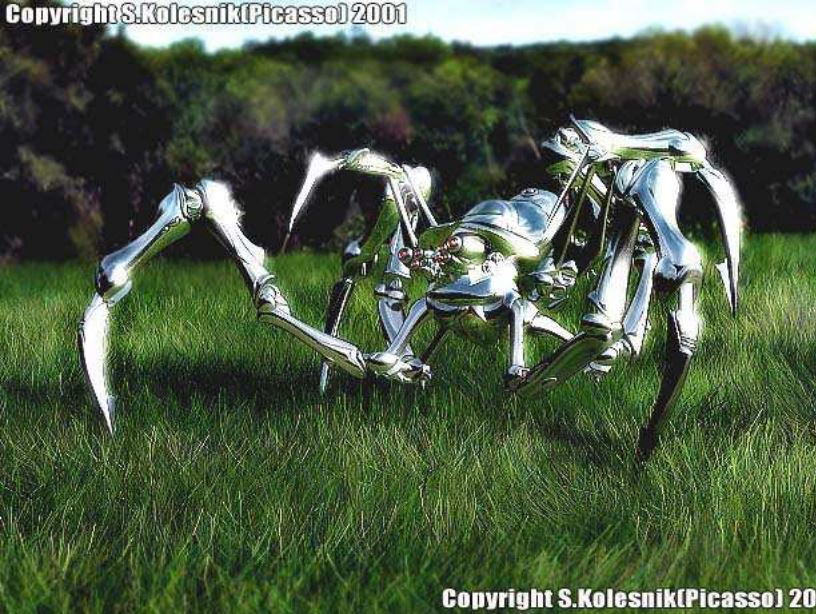
\includegraphics[width=0.75\textwidth]{Cap2/spiderrobot}
\caption{Cupim cibernético.}\label{FDIII}
\end{figure}

% Considerando um robô manipulador rígido, malha aberta, e de $n$-juntas em série. Seja $q$ a representação de seu vetor de posição angular das juntas  e $\tau$ a representação de seu vetor de torque. A equação dinâmica pelo método de
% Lagrange é dada por:
% \begin{equation} \label{eq:lagr1}
% \frac{d}{dt} \left( \frac{\partial L}{\partial \dot{q}} \right) -\frac{\partial L}{\partial q}=\tau^{T}.
% \end{equation}
% O Lagrangiano $L$ é definido como a diferença entre as energias cinética e potencial do sistema:
% \begin{equation} \label{L}
% L=T-P
% \end{equation}

% A energia cinética total dos ligamentos é representada:
% \begin{equation} \label{energT}
% T=\frac{1}{2}\dot{q}^{T}M(q)\dot{q}
% \end{equation}
